\PassOptionsToPackage{unicode=true}{hyperref} % options for packages loaded elsewhere
\PassOptionsToPackage{hyphens}{url}
\PassOptionsToPackage{dvipsnames,svgnames*,x11names*}{xcolor}
%
\documentclass[paper=a4,justified,a4paper]{tufte-handout}
\usepackage{lmodern}
\usepackage{amssymb,amsmath}
\usepackage{ifxetex,ifluatex}
\usepackage{fixltx2e} % provides \textsubscript
\ifnum 0\ifxetex 1\fi\ifluatex 1\fi=0 % if pdftex
  \usepackage[T1]{fontenc}
  \usepackage[utf8]{inputenc}
  \usepackage{textcomp} % provides euro and other symbols
\else % if luatex or xelatex
  \usepackage{unicode-math}
  \defaultfontfeatures{Ligatures=TeX,Scale=MatchLowercase}
\fi
% use upquote if available, for straight quotes in verbatim environments
\IfFileExists{upquote.sty}{\usepackage{upquote}}{}
% use microtype if available
\IfFileExists{microtype.sty}{%
\usepackage[]{microtype}
\UseMicrotypeSet[protrusion]{basicmath} % disable protrusion for tt fonts
}{}
\IfFileExists{parskip.sty}{%
\usepackage{parskip}
}{% else
\setlength{\parindent}{0pt}
\setlength{\parskip}{6pt plus 2pt minus 1pt}
}
\usepackage{xcolor}
\usepackage{hyperref}
\hypersetup{
            pdftitle={Evaluate your coaching skills - Reflection Report},
            pdfauthor={Helena Rasche},
            colorlinks=true,
            linkcolor=Maroon,
            filecolor=Maroon,
            citecolor=Blue,
            urlcolor=Blue,
            breaklinks=true}
\urlstyle{same}  % don't use monospace font for urls
\usepackage{longtable,booktabs}
% Fix footnotes in tables (requires footnote package)
\IfFileExists{footnote.sty}{\usepackage{footnote}\makesavenoteenv{longtable}}{}
\usepackage{graphicx,grffile}
\makeatletter
\def\maxwidth{\ifdim\Gin@nat@width>\linewidth\linewidth\else\Gin@nat@width\fi}
\def\maxheight{\ifdim\Gin@nat@height>\textheight\textheight\else\Gin@nat@height\fi}
\makeatother
% Scale images if necessary, so that they will not overflow the page
% margins by default, and it is still possible to overwrite the defaults
% using explicit options in \includegraphics[width, height, ...]{}
\setkeys{Gin}{width=\maxwidth,height=\maxheight,keepaspectratio}
\setlength{\emergencystretch}{3em}  % prevent overfull lines
\providecommand{\tightlist}{%
  \setlength{\itemsep}{0pt}\setlength{\parskip}{0pt}}
\setcounter{secnumdepth}{0}
% Redefines (sub)paragraphs to behave more like sections
\ifx\paragraph\undefined\else
\let\oldparagraph\paragraph
\renewcommand{\paragraph}[1]{\oldparagraph{#1}\mbox{}}
\fi
\ifx\subparagraph\undefined\else
\let\oldsubparagraph\subparagraph
\renewcommand{\subparagraph}[1]{\oldsubparagraph{#1}\mbox{}}
\fi

% set default figure placement to htbp
\makeatletter
\def\fps@figure{htbp}
\makeatother

\usepackage{pdfpages}

%%%%%%%%%%% Header and Footer %%%%%%%%%%%%%%%%%%
\fancyfoot[CE,CO]{\flushright 
\includegraphics[width=3cm]{../avans.jpg}}
\fancyhead[CE,CO]{\flushleft \smallcaps{\today}}


\title{Evaluate your coaching skills - Reflection Report}
\author{Helena Rasche}
\date{2022-02-07}

\begin{document}
\maketitle
\begin{abstract}
As the pandemic continues and lessons continue online, my primary
concern is that students are getting the support they need and feeling
supported. Following the experiences during BDB and with finally
beginning the period(s) during which I teach students, I've discovered a
number of points which I should remind myself of regularly as
preparation for each lesson.
\end{abstract}
\noindent\rule{5in}{0.4pt}


\hypertarget{points-of-attention}{%
\section{Points of Attention}\label{points-of-attention}}

Given that my lessons continue to be online, I find myself quite
concerned about whether or not students are getting enough support and
personal attention, and receiving it in ways that work optimally for
them. I know that students can feel significantly isolated with working
from home constantly, and that I want to ensure that I'm a friendly and
accepting person that they feel comfortable contacting when they have
issues. Specifically I've heard occasionally that I go too quickly and
sought their suggestions for how to fix this--I don't notice it unless
someone says it, and I'd rather they say it at the time it's happening.

\hypertarget{questionnaire}{%
\section{Questionnaire}\label{questionnaire}}

I designed the enquête to measure a couple aspects of this
communication:

\begin{itemize}
\tightlist
\item
  Preferred method(s)
\item
  Preferred interaction modalities
\item
  Their experiences as students in my class
\item
  And their feelings on my interactions with them until now.
\end{itemize}

These aspects I found to be particularly important to me and my
interactions with students. I elaborated these with the following survey
design:

\begin{longtable}[]{@{}lll@{}}
\toprule
\begin{minipage}[b]{0.09\columnwidth}\raggedright
Question\strut
\end{minipage} & \begin{minipage}[b]{0.14\columnwidth}\raggedright
Aspect\strut
\end{minipage} & \begin{minipage}[b]{0.68\columnwidth}\raggedright
Text\strut
\end{minipage}\tabularnewline
\midrule
\endhead
\begin{minipage}[t]{0.09\columnwidth}\raggedright
1\strut
\end{minipage} & \begin{minipage}[t]{0.14\columnwidth}\raggedright
Question\strut
\end{minipage} & \begin{minipage}[t]{0.68\columnwidth}\raggedright
How comfortable do you feel discussing course questions, issues,
programming questions via\strut
\end{minipage}\tabularnewline
\begin{minipage}[t]{0.09\columnwidth}\raggedright
1\strut
\end{minipage} & \begin{minipage}[t]{0.14\columnwidth}\raggedright
Description\strut
\end{minipage} & \begin{minipage}[t]{0.68\columnwidth}\raggedright
Example questions include: where's the course recording, why is my code
failing, what do you mean I need to import that first\strut
\end{minipage}\tabularnewline
\begin{minipage}[t]{0.09\columnwidth}\raggedright
1\strut
\end{minipage} & \begin{minipage}[t]{0.14\columnwidth}\raggedright
Answer\strut
\end{minipage} & \begin{minipage}[t]{0.68\columnwidth}\raggedright
A choice matrix of {[}Email, Teams Text Chat, Teams Video Chat, In
person{]} and {[}Please no!, If I must, Meh, It's ok, Yes please, My
preferred way!{]}\strut
\end{minipage}\tabularnewline
\begin{minipage}[t]{0.09\columnwidth}\raggedright
2\strut
\end{minipage} & \begin{minipage}[t]{0.14\columnwidth}\raggedright
Question\strut
\end{minipage} & \begin{minipage}[t]{0.68\columnwidth}\raggedright
I find online classes \ldots{}.\strut
\end{minipage}\tabularnewline
\begin{minipage}[t]{0.09\columnwidth}\raggedright
2\strut
\end{minipage} & \begin{minipage}[t]{0.14\columnwidth}\raggedright
Description\strut
\end{minipage} & \begin{minipage}[t]{0.68\columnwidth}\raggedright
1 = They work great for me! 5 = It's so exhausted I hate it here\strut
\end{minipage}\tabularnewline
\begin{minipage}[t]{0.09\columnwidth}\raggedright
2\strut
\end{minipage} & \begin{minipage}[t]{0.14\columnwidth}\raggedright
Answer\strut
\end{minipage} & \begin{minipage}[t]{0.68\columnwidth}\raggedright
Likert-type scale (1-5)\strut
\end{minipage}\tabularnewline
\begin{minipage}[t]{0.09\columnwidth}\raggedright
3\strut
\end{minipage} & \begin{minipage}[t]{0.14\columnwidth}\raggedright
Question\strut
\end{minipage} & \begin{minipage}[t]{0.68\columnwidth}\raggedright
How do you feel about\strut
\end{minipage}\tabularnewline
\begin{minipage}[t]{0.09\columnwidth}\raggedright
3\strut
\end{minipage} & \begin{minipage}[t]{0.14\columnwidth}\raggedright
Answer\strut
\end{minipage} & \begin{minipage}[t]{0.68\columnwidth}\raggedright
Choice matrix of {[}Breakout rooms, being randomly called on, being
predictably called on, Kahoots / Competitive quizzes{]} and feeling
matrix of {[}Hate it, Meh, It's fun{]}\strut
\end{minipage}\tabularnewline
\begin{minipage}[t]{0.09\columnwidth}\raggedright
4\strut
\end{minipage} & \begin{minipage}[t]{0.14\columnwidth}\raggedright
Question\strut
\end{minipage} & \begin{minipage}[t]{0.68\columnwidth}\raggedright
Helena wants to discuss my solution in front of the class, that makes me
feel\strut
\end{minipage}\tabularnewline
\begin{minipage}[t]{0.09\columnwidth}\raggedright
4\strut
\end{minipage} & \begin{minipage}[t]{0.14\columnwidth}\raggedright
Answer\strut
\end{minipage} & \begin{minipage}[t]{0.68\columnwidth}\raggedright
Free text\strut
\end{minipage}\tabularnewline
\begin{minipage}[t]{0.09\columnwidth}\raggedright
5\strut
\end{minipage} & \begin{minipage}[t]{0.14\columnwidth}\raggedright
Question\strut
\end{minipage} & \begin{minipage}[t]{0.68\columnwidth}\raggedright
Some of you have commented I go too quickly, how can we address
this?\strut
\end{minipage}\tabularnewline
\begin{minipage}[t]{0.09\columnwidth}\raggedright
5\strut
\end{minipage} & \begin{minipage}[t]{0.14\columnwidth}\raggedright
Description\strut
\end{minipage} & \begin{minipage}[t]{0.68\columnwidth}\raggedright
I'm guessing you don't want to publicly speak up? Would you want to
message the TOA who can ask me to slow down? Is there something I can do
to make you feel ok asking me to slow down in front of your peers? (I
need the reminder, I get too focused on covering content, for
sure.)\strut
\end{minipage}\tabularnewline
\begin{minipage}[t]{0.09\columnwidth}\raggedright
5\strut
\end{minipage} & \begin{minipage}[t]{0.14\columnwidth}\raggedright
Answer\strut
\end{minipage} & \begin{minipage}[t]{0.68\columnwidth}\raggedright
Free text\strut
\end{minipage}\tabularnewline
\begin{minipage}[t]{0.09\columnwidth}\raggedright
6\strut
\end{minipage} & \begin{minipage}[t]{0.14\columnwidth}\raggedright
Question\strut
\end{minipage} & \begin{minipage}[t]{0.68\columnwidth}\raggedright
I feel like part of the class when ?\strut
\end{minipage}\tabularnewline
\begin{minipage}[t]{0.09\columnwidth}\raggedright
6\strut
\end{minipage} & \begin{minipage}[t]{0.14\columnwidth}\raggedright
Description\strut
\end{minipage} & \begin{minipage}[t]{0.68\columnwidth}\raggedright
i.e.~specific types of activities (and that I'm getting something more
useful out of being here rather than doing chores or something
else.)\strut
\end{minipage}\tabularnewline
\begin{minipage}[t]{0.09\columnwidth}\raggedright
6\strut
\end{minipage} & \begin{minipage}[t]{0.14\columnwidth}\raggedright
Answer\strut
\end{minipage} & \begin{minipage}[t]{0.68\columnwidth}\raggedright
Free text\strut
\end{minipage}\tabularnewline
\begin{minipage}[t]{0.09\columnwidth}\raggedright
7\strut
\end{minipage} & \begin{minipage}[t]{0.14\columnwidth}\raggedright
Question\strut
\end{minipage} & \begin{minipage}[t]{0.68\columnwidth}\raggedright
Any other remarks?\strut
\end{minipage}\tabularnewline
\begin{minipage}[t]{0.09\columnwidth}\raggedright
7\strut
\end{minipage} & \begin{minipage}[t]{0.14\columnwidth}\raggedright
Answer\strut
\end{minipage} & \begin{minipage}[t]{0.68\columnwidth}\raggedright
Free text\strut
\end{minipage}\tabularnewline
\begin{minipage}[t]{0.09\columnwidth}\raggedright
8\strut
\end{minipage} & \begin{minipage}[t]{0.14\columnwidth}\raggedright
Question\strut
\end{minipage} & \begin{minipage}[t]{0.68\columnwidth}\raggedright
Are you getting the support you need? Do you have the resources you
need?\strut
\end{minipage}\tabularnewline
\begin{minipage}[t]{0.09\columnwidth}\raggedright
8\strut
\end{minipage} & \begin{minipage}[t]{0.14\columnwidth}\raggedright
Answer\strut
\end{minipage} & \begin{minipage}[t]{0.68\columnwidth}\raggedright
Likert-type scale with stars (1-5)\strut
\end{minipage}\tabularnewline
\begin{minipage}[t]{0.09\columnwidth}\raggedright
9\strut
\end{minipage} & \begin{minipage}[t]{0.14\columnwidth}\raggedright
Question\strut
\end{minipage} & \begin{minipage}[t]{0.68\columnwidth}\raggedright
Final Remarks?\strut
\end{minipage}\tabularnewline
\begin{minipage}[t]{0.09\columnwidth}\raggedright
9\strut
\end{minipage} & \begin{minipage}[t]{0.14\columnwidth}\raggedright
Answer\strut
\end{minipage} & \begin{minipage}[t]{0.68\columnwidth}\raggedright
Free text\strut
\end{minipage}\tabularnewline
\bottomrule
\end{longtable}

\hypertarget{results}{%
\subsection{Results}\label{results}}

\begin{figure}
\centering
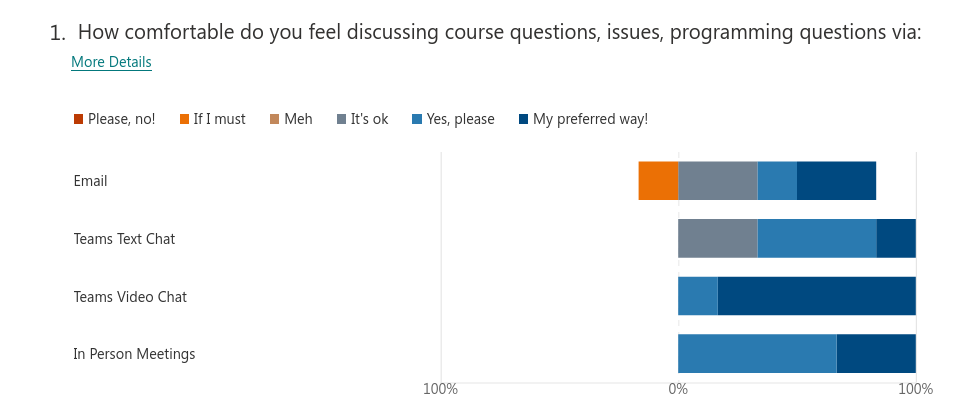
\includegraphics{./q1.png}
\caption{Students seem to be extremely comfortable with online
communication, many just want to see a face clearly as video chat was
rated even more highly than in-person meetings which is expected for my
section of students as they were the half of the class which did not
require in-person learning in a start of period survey.}
\end{figure}

Question 2 students overall rated online classes as an ok experience
(min=1, mean=2, max=4, sd=1), only one student gave a higher rating of 4
out of 5 (five being they're exhausted and hate it online), but this
shows suboptimal study design as I've conflated ``lack of enjoyment''
and ``exhaustion'' which I expect many of us are experiencing, and it's
unclear \emph{why} the student responded like they did.

\begin{figure}
\centering
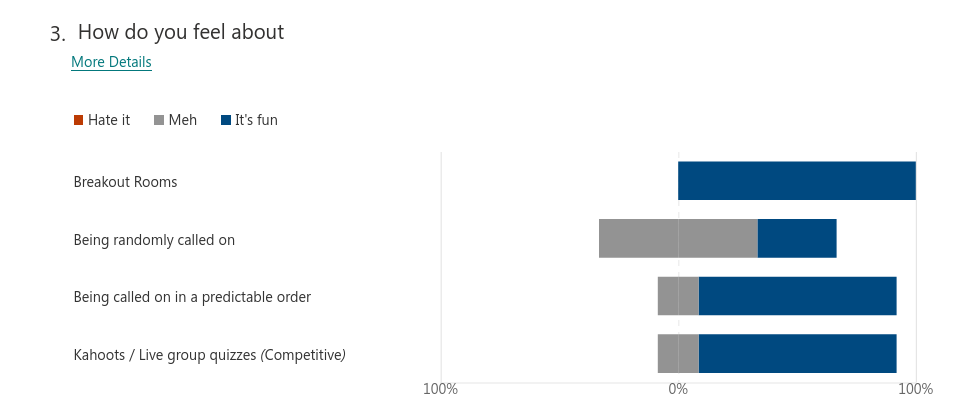
\includegraphics{./q3.png}
\caption{This question answers an important point for me, that students
are enjoying the new teaching methods implemented and discussed in
Assignment 10, breakout rooms where they do pair-programming.}
\end{figure}

Question 4's variety of responses have been interesting to say the
least. To summarize the main points of the students:

\begin{itemize}
\tightlist
\item
  Some worried because they were beginners, and know that their answer
  won't be correct.
\item
  Some feel very seen, that the teacher takes time to interact and
  discuss their answer.
\item
  Most felt ok with it, knowing that it was a necessary part of the
  learning process.
\end{itemize}

Seeing these responses, and given that this is a technical course where
we have a significant amount of control over where the students execute
code, I've asked my TOA to look into automating the collection of
student solutions to a given problem in a way that I can use it
dynamically during class. That will allow me to discuss student
solutions with the class anonymously and maybe achieve everyone's
objectives: no hurt feelings, no uncomfortable attention, and the
student's solutions we review will still feel seen.

Question 5 again gave food for thought on potential options to slow
down, some more actionable than others

\begin{itemize}
\tightlist
\item
  All steps should be repeated twice.
\item
  It's unclear when steps are something we need to run, or just for
  explanation.
\item
  I don't want to slow down just for me, knowing other people have the
  same issue helps
\item
  Sometimes you make a mistake, and catching up is tough, but the
  recording helps.
\item
  No problem with speed.
\end{itemize}

Question 6 interrogated their community spirit, in case there was
anything I could do to help there

\begin{itemize}
\tightlist
\item
  Answering questions together (x3)
\item
  Breakout rooms \& Exercises (x3)
\item
  People speak up
\end{itemize}

I really appreciated the insight of one student's response there:

\begin{quote}
People need to be more interactive. Nobody responds when you ask a
question. {[}\ldots{}{]} But I think it also can be frustrating for you
that nobody is responding.
\end{quote}

Which I have to concur with.

Question 7 had the most important point for me

\begin{itemize}
\tightlist
\item
  Lessons are great, sometimes a bit too fast
\item
  I really think you are a great teacher already to be honest!
\item
  I found it difficult to do the assignments with you 1:1, because I
  don't understand the assignments immediately and sometimes can feel
  like I am too slow.
\end{itemize}

That third point will be a focus of the reflection section below.

Question 8 showed students were absolutely getting the support they need
(min=4, max=5, mean=4.666, stdev=0.47)

Question 9 was the other remarks section and not well responded to which
is expected given that many people expressed opinions in 6.

\hypertarget{reflection}{%
\subsection{Reflection}\label{reflection}}

\begin{itemize}
\tightlist
\item
  communications ok
\item
  discuss problems with students
\item
  students need to hear others having those same issues before they're
  comfortable speaking up
\item
  difficult 1:1
\end{itemize}

\begin{enumerate}
\def\labelenumi{\arabic{enumi}.}
\setcounter{enumi}{3}
\tightlist
\item
  Process and describe the results and reflect on them via a reflection
  model of your choice.
\end{enumerate}

\hypertarget{action-points}{%
\section{Action Points}\label{action-points}}

\begin{itemize}
\tightlist
\item
  Go through questions at the end of each exercise section.
\item
  Go through student solutions anonymously and discuss common problems.
\item
  Do not pair with students, the knowledge gap is too significant,
  instead have them form trios.
\end{itemize}

\begin{enumerate}
\def\labelenumi{\arabic{enumi}.}
\setcounter{enumi}{4}
\tightlist
\item
  Formulate action points: to what and how do you want to work in
  relation to the teacher-student relationship?
\end{enumerate}

\end{document}
